\chapter{Literature Review \label{cha:litrev}}

This chapter focuses on the concepts that form the background of lifelong
learning and its link to universities. By discussing systems currently used in
the university environment, such as Learning Management Systems (LMS) and
ePortfolio system, the current state of the art is established and the need for
further development is outlined. This chapter focuses on the concepts that form
the background of lifelong learning and its link to universities. By discussing
systems currently used in the university environment, such as Learning
Management Systems (LMS) and ePortfolio system, the current state of the art is
established and the need for further development is outlined.

This chapter focuses on the concepts that form the background of lifelong
learning and its link to universities. By discussing systems currently used in
the university environment, such as Learning Management Systems (LMS) and
ePortfolio system, the current state of the art is established and the need for
further development is outlined. This chapter focuses on the concepts that form
the background of lifelong learning and its link to universities. By discussing
systems currently used in the university environment, such as Learning
Management Systems (LMS) and ePortfolio system, the current state of the art is
established and the need for further development is outlined.

\section{Literature Review Process}
The literature review to support and provide background for this project was
conducted by systematically reading and reviewing books, journals and conference
proceedings in the area of research. The main methods to identify relevant
literature were recommendations of domain experts and a library search. Relevant
articles were identified by reading titles and abstracts of selected journal
articles and papers in conference proceedings. Where possible the latest ten
years of issues of the following journals were looked through: ``British Journal
of Educational Technology'', ``International Journal of Lifelong Education'',
``European Journal of Education'', ``\LLLc in Europe'', ``International Journal
of Emerging Technologies in Learning'', ``New Zealand Journal of Adult
Learning'', ``Journal of Computer Assisted Learning'', ``European Journal of
Engineering Education'', and ``International Journal of ePortfolio''. In
addition, a keyword search was carried out on the Internet and academic
resources (such as Education Research
Complete\footnote{\url{http://www.ebscohost.com/academic/education-research-complete}},
Academic Search
Premier\footnote{\url{http://www.ebscohost.com/academic/academic-search-premier}},
Directory of Open Access Journals\footnote{\url{http://www.doaj.org}},
Google\footnote{\url{http://google.com}}, Google
Scholar\footnote{\url{http://scholar.google.com}}) to cover conference
publications not available in the library. The following keywords and
combinations of keywords were used in the search: ``\LLLsn'', ``life-long
learning'', ``e-learning'', ``ePortfolio'', ``e-portfolio'', and ``electronic
portfolio''.

This review helped to discover previous work in the area, explore methods
that could by applied to this research, increase the depth and breadth of
knowledge of the field, and identify domain experts and other people working
in the same field who could be valuable to contact. Besides finding relevant
information in the literature, it was also notable to identify the gaps that
currently exist. These gaps are based on facts that although a lot of work has
been done on developing \LLLs theories as well as developing technologies for
education and learning, there is little substantial work done on combining
these two areas. Reviewing the literature is a continuous process. Therefore,
the literature review for this research was updated by actively acquiring and
reading the relevant articles emerging in the literature.

\section{The General Concept of \LLLc}
The concept of \LLLs consists of a variety of meanings, models and ideas. Such
terms as '\LLLsn', 'lifelong education', 'adult education', 'recurrent
education', 'continuing education', and 'further education' create a set of
related yet different concepts \citep{Hager2011,Jarvis2004}.

The origin of the term '\LLLsn' goes back to the early 20th century and is
contributed to by John Dewey \citeyearpar{Dewey2004}. From his perspective,
\LLLs had to be centered on the individual's ability to take an active role in
democratic society. He saw education as a learning process which was influenced
by the growth of the individual and society, both interlinked. Dewey's key to
\LLLs was in developing active learning, enabling the individual to reflect and
change throughout life, emphasizing that non-formal education was as important
as formal education.

The concept of 'lifelong education' was discovered in 1972 after Edgar Faure's
Report ``Learning to Be'' for UNESCO. The concept described in the report was announced
to be the leading one for the reform in education. Faure's Report used four
principles for the lifelong education architecture \citep{Faure1972}: vertical
integration (education should occur throughout one's life), horizontal
integration (acceptance of non-formal and formal education), the democratization
of education (more widespread involvement of learners) and learning society
(restructuring of educational system). However, according to Hager's
\citeyearpar{Hager2011} analysis, UNESCO's concept of 'lifelong education' put
the emphasis on formal education as the only sufficient and relevant form of
learning to provide actual 'education'.

\begin{figure}[htb]
\centering
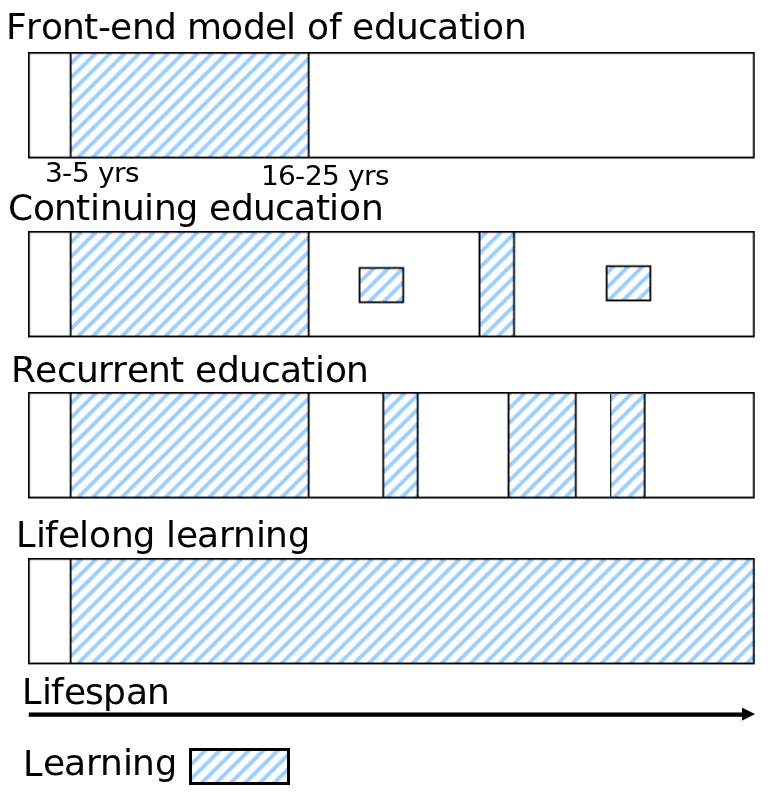
\includegraphics[width=0.6\textwidth]{CH3-F1-Learning}
\caption[Changing concepts of learning]{Changing concepts of learning 
\citep{Jarvis2004}}
\label{fig:learning}
\end{figure}

Now, almost 40 years after the idea of this lifelong education was introduced,
many governments rediscover not lifelong education, but \LLLs
\citep{Boshier2000}. This shift was not only semantic, but also substantive,
which showed that \LLLs and lifelong education are not the same: lifelong
education aimed to develop more humane individuals and communities, while
\LLLsn's goal is in retaining and learning new skills that would help
individuals adapt to rapid changes in their workplace
\citep{Medel-Anonuevo2001}. Lifelong learning is based on the notion of the
individual learner as a consumer. And as a result if consumers do not decide to
take advantage of all the opportunities they have – then it is their fault.
Therefore, being constructed as individual activity learning depends entirely on
personal motivation. Unlike learning, education is a provided service
(\citep{Boshier2000} that requires someone to be responsible for providing
resources, developing policies, etc. The emphasis on 'learning' rather than
'education' is significant \citep{Tuijnman2002}, as it moves focus from the
institutions onto the individual. But it does not mean that institutions and
govermnets play no role whatsoever. Their role is rather transformed into
investment in individuals and creation conditions for them to take charge of
their learning \citep{Chen2009}.

In terms of purposeful learning activities \LLLs consists of the following
components \citep{Longworth2003, Tuijnman2002}:

\begin{itemize}
  \item Formal learning (institutionally graded, and hierarchically structured
system, often leads to qualification);
  \item Non-formal learning (organized systematic educational activity external
to formal education);
  \item Informal learning (planned or not planned, but conscious learning from
the experience);
  \item Incidental learning (not intentional, an accompaniment to everyday life,
learning during the action).
\end{itemize} 

Some researchers recognize two categories of lifelong learning, formal and
non-formal, leaving informal and incidental parts of it as the elements of
non-formal learning \citep{Longworth2003}.

Boshier \citeyearpar{Boshier2000} states that at present the formal and non-formal
categories are like two parallel lines which seldom touch. Lifelong learning as well
encompasses the elements of self-direction, long-term and life-wide learning.
Therefore, it should also recognize the fact that learning also takes place
outside the formal education system and is guided by the learners themselves
\citep{Schuetze2006}. 

The European Commission defined Lifelong learning in its 2000 report
\citep{EuropeanCommission2000} as:

\longquote{All learning activity undertaken throughout life, with the aim of
improving knowledge, skills and competencies within a personal, civic, social
and/or employment-related perspective.} 

According to Rubenson (2002) the concept of \LLLs is based on fundamental
attributes:

\begin{itemize}
  \item It is lifelong and therefore concerns everything from cradle to grave;
  \item It is life-wide recognizing that learning occurs in many different
  settings and contexts;
  \item It self-directed and focuses on learning rather than limits itself to
education
\end{itemize} 

Some essential characteristics of \LLLs according to Weert and Kendall
\citeyearpar{Weert2004} also include:

\begin{itemize}
  \item Self-motivation as the driving force in \LLLsn;
  \item In \LLLs forms of progression and personal achievements are
  different;
  \item Lifelong learning is learner centred: demand driven and aiming for
  personal achievement;
  \item Lifelong learning will maintain a portfolio of personal achievement.
\end{itemize} 

\begin{figure}[htb]
\centering
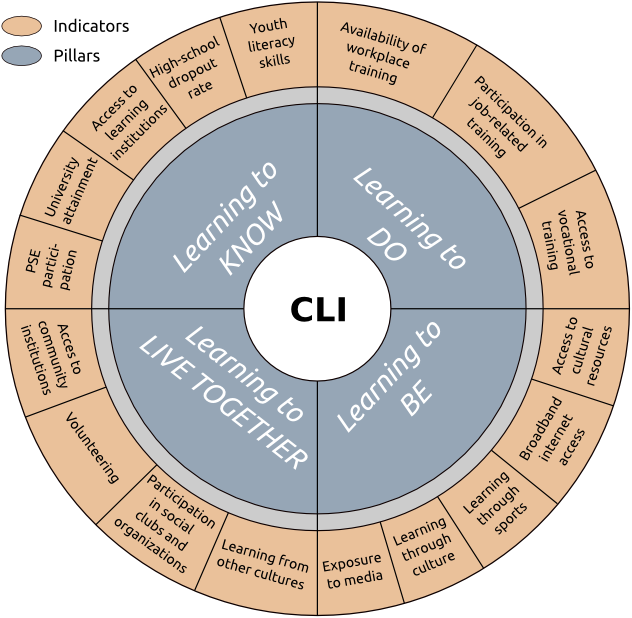
\includegraphics[width=0.8\textwidth]{CH3-F2-CLI}
\caption{The 2010 Composite Learning Index of Canada}
\label{fig:cli2010}
\end{figure}

Over recent years the skills that provide \LLLs ability were
identified, they include: solving problems, critical thinking, utilizing
technology, and information literacy; working with others in teams,
communication skills, leadership and social interaction skills; self-management;
collecting, analyzing and organizing information; planning and organizing
activities; cultural awareness and understanding
\citep{Brooks2008,Heinrich2007,Otala1997,Pitman2009}.

\section{\LLLc in Universities}

As lifelong learning consists of the concepts of 'life-long', 'life-wide' and
'self- directed' learning, it has following significant implications. In the
broadest sense 'life-long' means the full life span of an individual. From the
institutional view it starts when students are enrolled in the university and
finishes when they graduate. 'Life-wide' learning implies that learning can and
should occur not only as formal university study, as personal and professional
development takes place in many contexts. Attwell \citeyearpar{Attwell2007}
considers the fact that everyday non-formal types of learning are not connected
to institutional formal education to be the major issue of modern learning,
which can make students see their study at university as ``something irrelevant
to their identities'' (p. 4). For successful lifelong learning, progress of the
achievements should be recorded and maintained over a long period and across
various sources, formal as well as non-formal \citep{Kay2008}. A lifelong
learning environment needs to acknowledge this and allow learners to record and
reflect on experiences from all these contexts.

The importance of lifelong learning skills in addition to academic and subject
knowledge has been increasingly emphasised in the workplace and public policy
over the last decade \citep{Morgan-Klein2007,Sutherland2006}. Individuals today
need to continue to update and upgrade their skills and knowledge even after
completing formal education in order to survive in the changing world. Otala
\citeyearpar{Otala1997} states that required flexibility and adaptability to these
rapid changes are gained through ``better developed learning skills and the
right attitudes that help individuals quickly and easily learn new things'' (p.
456).

Therefore, current students need to ``possess something more than skills which
grow obsolete as technology advances'' \cite[p.~195]{Field2003}. Higher
education institutions have responded to this need defining their own strategies
to promote \LLLsn. A number of universities in Europe, the United
States, Australia and New Zealand now express the \LLLs characteristics they
strive for in their graduates \citep{Scanlon2006}. Some Australian universities,
for example Curtin University, went as far as officially declaring their own
policies committing to produce graduates who demonstrate the required graduate
attributes (Curtin University, 2006). In some universities, particular programs
try to meet institutional needs to promote \LLLsn in more coherent
manner on department level. For example, the College of Sciences of Massey
University has formulated a draft lifelong learning policy (Massey University,
2008) that expresses values, support and expectations in regards to \LLLsn.
Graduate profiles, naming lifelong learning skills such as critical thinking,
effective communication, teamwork, leadership have been established for many
degree programmes (Davies and LeMahieu, 2003; McAlister and Alexander, 2003).

\section{Requirements for Successful \LLLc}
 
Literature identifies a number of requirements that have to be satisfies in
order to achieve successful lifelong learning support.
 
\begin{itemize}
  \item Universities should provide support for all aspects of learning (formal,
  informal, etc.); 
  \item Students need guidance on various levels \citep{Leone2019};
  \item Lecturer should be an active facilitator and promote involving learning
experiences \citep{Leone2019}; 
  \item Communication and collaboration are essential parts of learning process
  \citep{Schaffert2008};
  \item Progress of the achievements should be recorded from various sources and
maintained over a long period of time \citep{Kay2008}; 
  \item Students need to be aware of their personal achievements
\citep{Schuetze2006};
  \item Students should develop understanding and confidence in their knowledge
  and be able to address higher-order skills (graduate attributes in university
  context) \citep{Hart1999};
  \item Students should be able to evaluate and reflect on their own performance
and learning progress \citep{Mourtos2003};
\end{itemize} 

\section{Summary} 